\documentclass[8pt]{extarticle}
\title{}
\author{Avinash Iyer}
\date{}

%font setup
%
%\usepackage[math]{anttor}

%paper setup
\usepackage{geometry}
\geometry{letterpaper, portrait, margin=1in}
\usepackage{fancyhdr}

%symbols
\usepackage{amsmath}
\usepackage{amssymb}
\usepackage{hyperref}
\usepackage{gensymb}

\usepackage[T1]{fontenc}
\usepackage[utf8]{inputenc}

%chemistry stuff
\usepackage[version=4]{mhchem}
\usepackage{chemfig}

%plotting
\usepackage{pgfplots}
\usepackage{tikz}

%\usepackage{natbib}

%graphics stuff
\usepackage{graphicx}
\graphicspath{ {./images/} }

%a useful command
\newcommand{\plain}[1]{\textrm{#1}}

%code stuff
%when using minted, make sure to add the -shell-escape flag
%you can use lstlisting if you don't want to use minted
%\usepackage{minted}
%\usemintedstyle{pastie}
%\newminted[javacode]{java}{frame=lines,framesep=2mm,linenos=true,fontsize=\footnotesize,tabsize=3,autogobble,}
%\newminted[cppcode]{cpp}{frame=lines,framesep=2mm,linenos=true,fontsize=\footnotesize,tabsize=3,autogobble,}

\usepackage{listings}
\usepackage{color}
\definecolor{dkgreen}{rgb}{0,0.6,0}
\definecolor{gray}{rgb}{0.5,0.5,0.5}
\definecolor{mauve}{rgb}{0.58,0,0.82}

\lstset{frame=tb,
	language=Java,
	aboveskip=3mm,
	belowskip=3mm,
	showstringspaces=false,
	columns=flexible,
	basicstyle={\small\ttfamily},
	numbers=none,
	numberstyle=\tiny\color{gray},
	keywordstyle=\color{blue},
	commentstyle=\color{dkgreen},
	stringstyle=\color{mauve},
	breaklines=true,
	breakatwhitespace=true,
	tabsize=3
}
\pagestyle{fancy}
\fancyhf{}
\rhead{Avinash Iyer, Tobias Searcy-Jorgensen}
\lhead{Lab 5: Centripetal Acceleration}
\pgfplotsset{every tick label/.append style={font=\tiny}}
\begin{document}{
\section*{Abstract}%
\label{sec:Abstract}
The experiment performed in this lab attempted to test a relation between a mass in uniform circular motion $m_1$ threaded through a straw with a mass $m_2$ on the other end, the period of the swings, $T$, and the length $L$. A rubber stopper was knotted through one end of a string, with $1.00\pm 0.01$m measured out on the string and marked with a bright marker. After measuring out $1.00$m on the thread, an extra 20cm was added and the string was threaded through a straw, with a variety of measured out washers serving as a varying $m_2$. We went to an open area, kept the $1.00$m length on the top end of the straw, and attached an alligator clip $1$cm below the straw to serve as a guide. After attaching the alligator clip, we swung the top end of the string with a rubber stopper around, and measured out 10 rotations. The expected slope of a graph with $T^2$ on the $y$ axis and $1/m_{2}$ on the $x$ axis, using a length $L = 1.00 \pm 0.01$m, $g = 9.8$m/s$^2$, and $m_1 = 10.8\pm 0.05$g, was $43.5\pm 0.5$. After performing the experiment with $m_2$ ranging between $6.2$ and $63.1$ grams, we found that there were $5$ outliers among the lower set of data values, primarily due to difficulties in performing the given test. The value of the slope of the regression line for the remaining set of values was $45$, with a $y$ intercept of $-0.2$, which was not consistent with the expected value. This was likely due to errors in finding the period of the rotation, difficulties in experiment execution (which while lessened with higher masses, was still a not insignificant factor), and other random uncertainties that were magnified through the experiment process.
\section*{Quantitative Prediction}
\subsection*{Part A}
\begin{quote}
	Decide which quantities should be plotted on the axes of a graph so that the expected graph will be a straight line that passes through the origin. (Hint: These quantities should only be functions of varied quantities that are in the formula, and not include any constants). Express the slope of this line in terms of other quantities that are in the formula. Check the result with your instructor.
\end{quote}
We will plot the value of $T^{2}$ on the $y$ axis and $\frac{1}{m_2}$ on the $x$ axis. This will yield a graph with slope $\frac{4\pi^2Lm_1}{g}$.
\subsection*{Part B}
\begin{quote}
	Measure the quantities that appear in the slope, and evaluate their uncertainties. Be sure to carefully consider all types of uncertainties that may be present in any particular measurement, including instrumental uncertainties, random uncertainties, and those caused by a problem of definition.  (Hint: It may be helpful for you to perform a few trials first in order to evaluate the difficulty keeping the value of L constant at exactly 1 meter). Report the measurements and their uncertainties, and explain the sources of uncertainty in each measurement.
\end{quote}
\begin{itemize}
	\item $m_1 = 10.8 \pm 0.05$ g, primarily from instrumental uncertainty.
	\item $L = 1.00 \pm 0.01$ m, primarily from random uncertainties and problem of definition. Though the direct measurement of $L$ was possible to a precision of $0.001$ m, random uncertainties in how to regard the distances amplified the uncertainty to $0.01$ m.
\end{itemize}
\subsection*{Part C}
\begin{quote}
	Use these measurements to calculate the expected value of the slope and the uncertainty in the expected value of the slope using the appropriate rules for uncertainty propagation. Show all your calculations. Report the calculated slope along with its uncertainty in an appropriate format. This is your predicted slope.
\end{quote}
\begin{align*}
	T^2 &= a\left(\frac{1}{m_2}\right) \\
	a &= \frac{4\pi^2Lm_1}{g} \\
	&= \frac{4\pi^2(1)(10.8)}{9.8} \\
	&= 43.5 \\
	\delta a &= a \sqrt{\left(\frac{\delta L}{L}\right)^2 + \left(\frac{\delta m_1}{m_1}\right)^2} \\
	&= 0.5 \\
	a &= 43.5 \pm 0.5
\end{align*}
\subsection*{Part D}
\begin{quote}
	The expected graph was a straight line.  What is its predicted intercept?
\end{quote}
The predicted intercept of the graph is $(0,0)$, as there is no constant function that should affect the $T$ or $T^2$ term.
\section*{Procedures}
\subsection*{Part A}
\begin{quote}
	Design and describe in detail the experiment that you will perform in order to test whether or not Eq. [1] accurately describes the physical situation. Include a labeled sketch of the design of the experiment. Decide which physical quantities you have to measure and how you are going to measure them.
\end{quote}
The participant will measure the mass of the rubber stopper in grams on a triple beam balance as well as a sequentially larger set of washers to serve as the mass attached to the lower end of the string. The participant will then tie the rubber stopper to one end of a string, and measure out $1.00$ m of string with a meter stick, and mark the end with a bright permanent marker. After marking the edge of the string, the participant will then roll out another length of string to remain within the straw and attach washers, and cut the string to the desired length. The participant will thread the string through the straw, and on the end of the string on the other side of the rubber stopper, tie the requisite number of washers. The participants will also attach an alligator clip approximately 0.5 cm below the straw when the marked end of the string is at the top edge of the straw. The participant will then move to an open area far away from other people or objects, and throw the rubber stopper end above their head in circular motion. The alligator clip should not touch the bottom of the straw, and the marked edge of the string must be located at the tip of the straw. The participant's partner will measure out ten rotations of the stopper and time them on their stopwatch.
\subsection*{Part B}
\begin{quote}
	Show how to convert the measured quantities into the quantities plotted on the axes of the graph.
\end{quote}
The value of $T$ should be squared, and plotted along the $y$ axis, while the value of $m$ should be inverted and plotted along the $x$ axis.
\subsection*{Part C}
The uncertainties in the measured quantities $\delta T$ and $\delta m$ should be plotted via the following:
\begin{align*}
	\label{eq:}
	\delta \left(T^2\right) &= 2T\delta T \\
	\delta \left(\frac{1}{m}\right) &= \frac{\delta m}{m^2}
\end{align*}
\subsection*{Part D}
\begin{quote}
	Give a list of assumptions to be made in order to solve the problem, with clear explanations of how these assumptions affect the results.
\end{quote}
\begin{itemize}
	\item Zero air resistance or friction: If there is friction, our results will be skewed towards lower periods, and so will shift our measured slope downward.
	\item Length of string is $1$m: If the length of the string is longer than $1$, the measured slope will be higher than the actual slope.
	\item The rotations are consistent: If the rotations are not consistent, or the alligator clip touches the bottom of the straw, then the period measurements will be shifted downward as the straw would be able to sustain a faster period than the value of $m_2$ would suggest.
\end{itemize}
\subsection*{Part E}%
\label{sub:Part E}
\begin{itemize}
	\item $\delta T$: This will be minimized by measuring the time for 10 rotations and dividing by 10.
	\item $\delta m_1$: This is minimized by using the triple beam balance.
	\item $\delta m_2$: This is minimized by using the triple beam balance.
\end{itemize}
\section*{Data}
\subsection*{Part A}%
\label{sub:Part A}

\begin{center}
	\begin{tabular}{c|c}
		Quantity & Measurement with Uncertainty \\
		\hline
		$m_1$ & $10.8 \pm 0.05$g\\
		$L$ & $1.00 \pm 0.01$m \\
		\hline
		\hline
		$m_{21}$ & $6.2 \pm 0.05$g \\
		$10T_1$ & $14.42 \pm 0.5$s \\
		\hline
		$m_{22}$ & $12.6 \pm 0.05$g \\
		$11T_2$ & $13.69 \pm 0.5$s \\
		\hline
		$m_{23}$ & $19.5 \pm 0.05$g \\
		$10T_3$ & $13.45 \pm 0.5$s \\
		\hline
		$m_{24}$ & $25.7 \pm 0.05$g \\
		$10T_4$ & $11.29 \pm 0.5$s \\
		\hline
		$m_{25}$ & $32.0 \pm 0.05$g \\
		$10T_{5}$ & $10.77 \pm 0.5$s \\
		\hline
		$m_{26}$ & $38.6 \pm 0.05$g \\
		$10T_{6}$ & $10.27 \pm 0.5$s \\
		\hline
		$m_{27}$ & $44.5\pm 0.05$g \\
		$10T_{7}$ & $8.94 \pm 0.5$s \\
		\hline
		$m_{28}$ & $50.8 \pm 0.05$g \\
		$10T_{8}$ & $8.20 \pm 0.5$s \\
		\hline
		$m_{29}$ & $56.9 \pm 0.05$g \\
		$10T_9$ & $7.54 \pm 0.5$s \\
		\hline
		$m_{210}$ & $63.1 \pm 0.05$g \\
		$10T_{10}$ & $7.21 \pm 0.5$s
	\end{tabular}
\end{center}
\subsection*{Part B}%
\label{sub:Part B}
\begin{align*}
	\label{eq:}
	10T_1 &= 14.42 \\
	T_1 &= 1.44 \\
	T_1^2 &= 2.07 \\
	\delta\left(10T_1\right) &= 0.5 \\
	\delta T_1 &= 0.05 \\
	\delta\left(T_1^2\right) &= 2T_1\delta T_1\\
	&= 0.2 \\
	m_{21} &= 6.2 \\
	\frac{1}{m_{21}} &= 0.16 \\
	\delta m_{21} &= 0.05 \\
	\delta \frac{1}{m_{21}} &= \frac{\delta m_{21}}{m_{21}^2} \\
	&= 0.01
\end{align*}
\section*{Data Analysis}%
\label{sec:Data Analysis}
\subsection*{Part A}%
\label{sub:Part A}

\begin{center}
	\resizebox{12cm}{!}{
	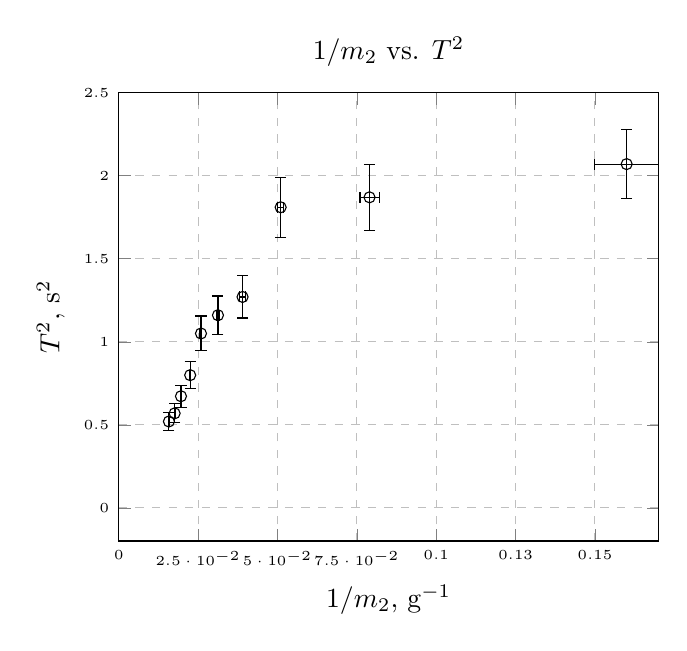
\begin{tikzpicture}
		\begin{axis}[
			title={$1/m_{2}$ vs. $T^2$},
			xlabel={$1/m_2$, g$^{-1}$},
			ylabel={$T^2$, s$^2$},
			xmin = 0, xmax = 0.17,
			ymin=-0.2, ymax = 2.5,
			xtick={0,0.025,0.050,0.075,0.100,0.125,0.150},
			ytick={0,0.5,1,1.5,2,2.5},
			xmajorgrids=true, ymajorgrids=true, grid style = dashed,
			]
			\addplot[only marks, mark = o, error bars/.cd, y dir = both, x dir = both, x explicit, y explicit] coordinates {
				(0.16,2.07) +- (0.01,0.207)
				(0.079, 1.87) +- (0.003,0.2)
				(0.051,1.81) +- (0.001,0.181)
				(0.039,1.27) +- (0.001,0.127)
				(0.03125,1.16) +- (0.0005,0.116)
				(0.0259,1.05) +- (0.0003,0.105)
				(0.0225,0.799) +- (0.0002,0.0799)
				(0.0196,0.672) +- (0.0002,0.0672)
				(0.0176,0.569) +- (0.00015,0.0569)
				(0.0158,0.520) +- (0.0001,0.0519)
			};
		\end{axis}
	\end{tikzpicture}
	}
\end{center}
The graph is not linear over the entire data range.
\subsection*{Part B}%
\label{sub:Part B}
The range of $m_2$ between $32.0$ and $63.1$ grams yields a linear result. The fractional uncertainty among smaller values of $m_2$ is larger in the first place, and while performing the experiment with small values of $m_2$, one of the experimental assumptions (that the alligator clip is not touching the bottom of the straw) is likely violated, depressing the value of $T^2$ for these values.
\subsection*{Part C}%
\label{sub:Part C}
\begin{center}
	\resizebox{12cm}{!}{
	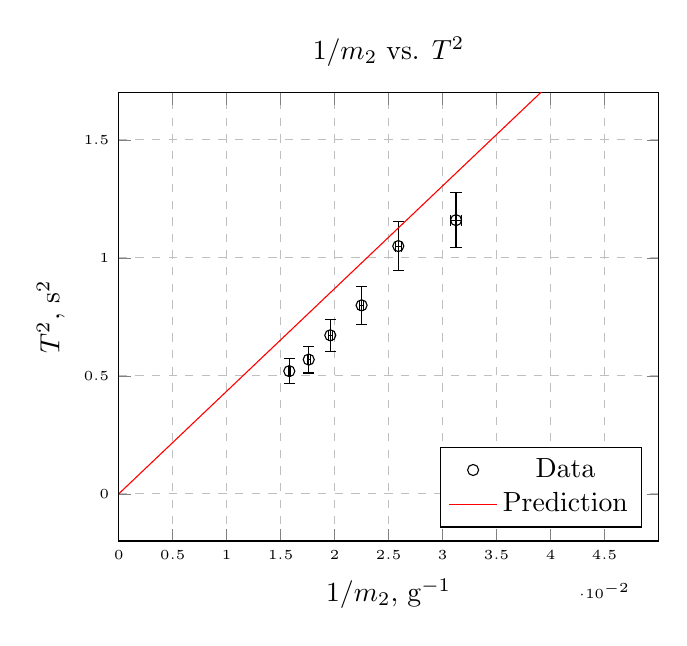
\begin{tikzpicture}
		\begin{axis}[
			title={$1/m_{2}$ vs. $T^2$},
			xlabel={$1/m_2$, g$^{-1}$},
			ylabel={$T^2$, s$^2$},
			xmin = 0, xmax = 0.05,
			ymin=-0.2, ymax = 1.7,
			xtick={0,0.005,0.010,0.015,0.020,0.025,0.030,0.035,0.040,0.045},
			ytick={0,0.5,1,1.5},
			xmajorgrids=true, ymajorgrids=true, grid style = dashed,
			legend pos = south east
			]
			\addplot[only marks, mark = o, error bars/.cd, y dir = both, x dir = both, x explicit, y explicit] coordinates {
				(0.03125,1.16) +- (0.0005,0.116)
				(0.0259,1.05) +- (0.0003,0.105)
				(0.0225,0.799) +- (0.0002,0.0799)
				(0.0196,0.672) +- (0.0002,0.0672)
				(0.0176,0.569) +- (0.00015,0.0569)
				(0.0158,0.520) +- (0.0001,0.0519)
			};
			\addlegendentry{Data}
			\addplot [domain = 0:0.05,samples=100,color=red]{(43.5)*x};
			\addlegendentry{Prediction}
		\end{axis}
	\end{tikzpicture}
	}
\end{center}
\subsection*{Part D}%
\label{sub:Part D}
After performing the linear regression on the selected data, we get a slope of $45$ with a $y$-intercept of $-0.2$. This is \textbf{not} within the margin of error for $m$ in our quantitative prediction. The graph is on the following page.
\begin{center}
	\resizebox{12cm}{!}{
	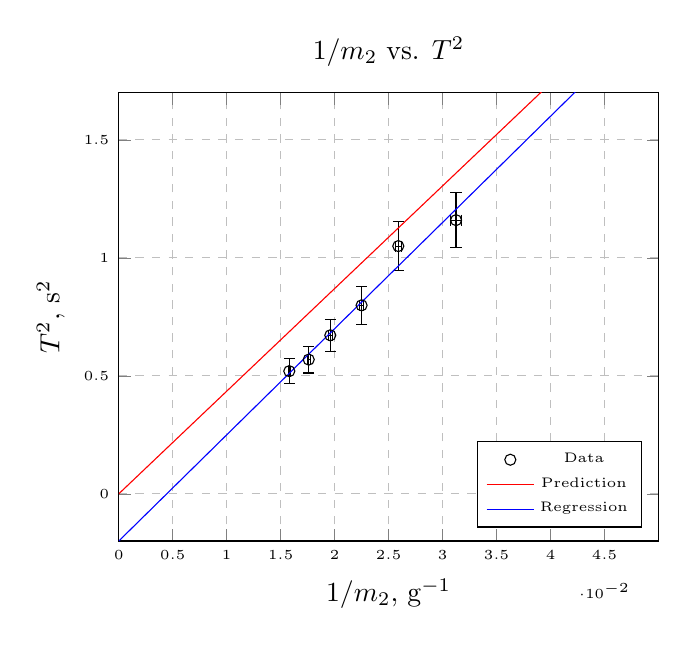
\begin{tikzpicture}
		\begin{axis}[
			title={$1/m_{2}$ vs. $T^2$},
			xlabel={$1/m_2$, g$^{-1}$},
			ylabel={$T^2$, s$^2$},
			xmin = 0, xmax = 0.05,
			ymin=-0.2, ymax = 1.7,
			xtick={0,0.005,0.010,0.015,0.020,0.025,0.030,0.035,0.040,0.045},
			ytick={0,0.5,1,1.5},
			xmajorgrids=true, ymajorgrids=true, grid style = dashed,
			legend pos = south east
			]
			\addplot[only marks, mark = o, error bars/.cd, y dir = both, x dir = both, x explicit, y explicit] coordinates {
				(0.03125,1.16) +- (0.0005,0.116)
				(0.0259,1.05) +- (0.0003,0.105)
				(0.0225,0.799) +- (0.0002,0.0799)
				(0.0196,0.672) +- (0.0002,0.0672)
				(0.0176,0.569) +- (0.00015,0.0569)
				(0.0158,0.520) +- (0.0001,0.0519)
			};
			\addlegendentry{\tiny Data}
			\addplot [domain = 0:0.05,samples=100,color=red]{(43.5)*x};
			\addlegendentry{\tiny Prediction}
			\addplot[domain=0:0.05,samples=100,color=blue]{(45)*x - 0.2};
			\addlegendentry{\tiny Regression}
		\end{axis}
	\end{tikzpicture}
	}
\end{center}
\subsection*{Part E}%
\label{sub:Part E}
It is likely that the following experimental factors yielded a slope that was inconsistent with the prediction:
\begin{itemize}
	\item Alligator clip: The alligator clip does not have negligible mass, and we failed to account for this in our measurements of the various masses.
	\item Clip touches bottom of straw: Even while taking care to avoid the alligator clip touching the bottom of the straw and removing data points where it did touch the bottom of the straw, it is likely the clip did touch the bottom of the straw, which severely distorted the data.
	\item Errors in calculating period: It is possible that the human error in finding the period was larger than the $0.5$s that was assumed.
\end{itemize}
}\end{document}
